\documentclass[]{book}
\usepackage{lmodern}
\usepackage{amssymb,amsmath}
\usepackage{ifxetex,ifluatex}
\usepackage{fixltx2e} % provides \textsubscript
\ifnum 0\ifxetex 1\fi\ifluatex 1\fi=0 % if pdftex
  \usepackage[T1]{fontenc}
  \usepackage[utf8]{inputenc}
\else % if luatex or xelatex
  \ifxetex
    \usepackage{mathspec}
  \else
    \usepackage{fontspec}
  \fi
  \defaultfontfeatures{Ligatures=TeX,Scale=MatchLowercase}
\fi
% use upquote if available, for straight quotes in verbatim environments
\IfFileExists{upquote.sty}{\usepackage{upquote}}{}
% use microtype if available
\IfFileExists{microtype.sty}{%
\usepackage{microtype}
\UseMicrotypeSet[protrusion]{basicmath} % disable protrusion for tt fonts
}{}
\usepackage[margin=1in]{geometry}
\usepackage{hyperref}
\hypersetup{unicode=true,
            pdftitle={An Introduction to Machine Learning},
            pdfauthor={Sudhakaran Prabakaran, Matt Wayland and Chris Penfold},
            pdfborder={0 0 0},
            breaklinks=true}
\urlstyle{same}  % don't use monospace font for urls
\usepackage{natbib}
\bibliographystyle{apalike}
\usepackage{color}
\usepackage{fancyvrb}
\newcommand{\VerbBar}{|}
\newcommand{\VERB}{\Verb[commandchars=\\\{\}]}
\DefineVerbatimEnvironment{Highlighting}{Verbatim}{commandchars=\\\{\}}
% Add ',fontsize=\small' for more characters per line
\usepackage{framed}
\definecolor{shadecolor}{RGB}{248,248,248}
\newenvironment{Shaded}{\begin{snugshade}}{\end{snugshade}}
\newcommand{\KeywordTok}[1]{\textcolor[rgb]{0.13,0.29,0.53}{\textbf{{#1}}}}
\newcommand{\DataTypeTok}[1]{\textcolor[rgb]{0.13,0.29,0.53}{{#1}}}
\newcommand{\DecValTok}[1]{\textcolor[rgb]{0.00,0.00,0.81}{{#1}}}
\newcommand{\BaseNTok}[1]{\textcolor[rgb]{0.00,0.00,0.81}{{#1}}}
\newcommand{\FloatTok}[1]{\textcolor[rgb]{0.00,0.00,0.81}{{#1}}}
\newcommand{\ConstantTok}[1]{\textcolor[rgb]{0.00,0.00,0.00}{{#1}}}
\newcommand{\CharTok}[1]{\textcolor[rgb]{0.31,0.60,0.02}{{#1}}}
\newcommand{\SpecialCharTok}[1]{\textcolor[rgb]{0.00,0.00,0.00}{{#1}}}
\newcommand{\StringTok}[1]{\textcolor[rgb]{0.31,0.60,0.02}{{#1}}}
\newcommand{\VerbatimStringTok}[1]{\textcolor[rgb]{0.31,0.60,0.02}{{#1}}}
\newcommand{\SpecialStringTok}[1]{\textcolor[rgb]{0.31,0.60,0.02}{{#1}}}
\newcommand{\ImportTok}[1]{{#1}}
\newcommand{\CommentTok}[1]{\textcolor[rgb]{0.56,0.35,0.01}{\textit{{#1}}}}
\newcommand{\DocumentationTok}[1]{\textcolor[rgb]{0.56,0.35,0.01}{\textbf{\textit{{#1}}}}}
\newcommand{\AnnotationTok}[1]{\textcolor[rgb]{0.56,0.35,0.01}{\textbf{\textit{{#1}}}}}
\newcommand{\CommentVarTok}[1]{\textcolor[rgb]{0.56,0.35,0.01}{\textbf{\textit{{#1}}}}}
\newcommand{\OtherTok}[1]{\textcolor[rgb]{0.56,0.35,0.01}{{#1}}}
\newcommand{\FunctionTok}[1]{\textcolor[rgb]{0.00,0.00,0.00}{{#1}}}
\newcommand{\VariableTok}[1]{\textcolor[rgb]{0.00,0.00,0.00}{{#1}}}
\newcommand{\ControlFlowTok}[1]{\textcolor[rgb]{0.13,0.29,0.53}{\textbf{{#1}}}}
\newcommand{\OperatorTok}[1]{\textcolor[rgb]{0.81,0.36,0.00}{\textbf{{#1}}}}
\newcommand{\BuiltInTok}[1]{{#1}}
\newcommand{\ExtensionTok}[1]{{#1}}
\newcommand{\PreprocessorTok}[1]{\textcolor[rgb]{0.56,0.35,0.01}{\textit{{#1}}}}
\newcommand{\AttributeTok}[1]{\textcolor[rgb]{0.77,0.63,0.00}{{#1}}}
\newcommand{\RegionMarkerTok}[1]{{#1}}
\newcommand{\InformationTok}[1]{\textcolor[rgb]{0.56,0.35,0.01}{\textbf{\textit{{#1}}}}}
\newcommand{\WarningTok}[1]{\textcolor[rgb]{0.56,0.35,0.01}{\textbf{\textit{{#1}}}}}
\newcommand{\AlertTok}[1]{\textcolor[rgb]{0.94,0.16,0.16}{{#1}}}
\newcommand{\ErrorTok}[1]{\textcolor[rgb]{0.64,0.00,0.00}{\textbf{{#1}}}}
\newcommand{\NormalTok}[1]{{#1}}
\usepackage{longtable,booktabs}
\usepackage{graphicx,grffile}
\makeatletter
\def\maxwidth{\ifdim\Gin@nat@width>\linewidth\linewidth\else\Gin@nat@width\fi}
\def\maxheight{\ifdim\Gin@nat@height>\textheight\textheight\else\Gin@nat@height\fi}
\makeatother
% Scale images if necessary, so that they will not overflow the page
% margins by default, and it is still possible to overwrite the defaults
% using explicit options in \includegraphics[width, height, ...]{}
\setkeys{Gin}{width=\maxwidth,height=\maxheight,keepaspectratio}
\IfFileExists{parskip.sty}{%
\usepackage{parskip}
}{% else
\setlength{\parindent}{0pt}
\setlength{\parskip}{6pt plus 2pt minus 1pt}
}
\setlength{\emergencystretch}{3em}  % prevent overfull lines
\providecommand{\tightlist}{%
  \setlength{\itemsep}{0pt}\setlength{\parskip}{0pt}}
\setcounter{secnumdepth}{5}
% Redefines (sub)paragraphs to behave more like sections
\ifx\paragraph\undefined\else
\let\oldparagraph\paragraph
\renewcommand{\paragraph}[1]{\oldparagraph{#1}\mbox{}}
\fi
\ifx\subparagraph\undefined\else
\let\oldsubparagraph\subparagraph
\renewcommand{\subparagraph}[1]{\oldsubparagraph{#1}\mbox{}}
\fi

%%% Use protect on footnotes to avoid problems with footnotes in titles
\let\rmarkdownfootnote\footnote%
\def\footnote{\protect\rmarkdownfootnote}

%%% Change title format to be more compact
\usepackage{titling}

% Create subtitle command for use in maketitle
\newcommand{\subtitle}[1]{
  \posttitle{
    \begin{center}\large#1\end{center}
    }
}

\setlength{\droptitle}{-2em}
  \title{An Introduction to Machine Learning}
  \pretitle{\vspace{\droptitle}\centering\huge}
  \posttitle{\par}
  \author{Sudhakaran Prabakaran, Matt Wayland and Chris Penfold}
  \preauthor{\centering\large\emph}
  \postauthor{\par}
  \predate{\centering\large\emph}
  \postdate{\par}
  \date{2017-09-01}

\usepackage{booktabs}
\usepackage{amsthm}
\makeatletter
\def\thm@space@setup{%
  \thm@preskip=8pt plus 2pt minus 4pt
  \thm@postskip=\thm@preskip
}
\makeatother

\usepackage{amsthm}
\newtheorem{theorem}{Theorem}[chapter]
\newtheorem{lemma}{Lemma}[chapter]
\theoremstyle{definition}
\newtheorem{definition}{Definition}[chapter]
\newtheorem{corollary}{Corollary}[chapter]
\newtheorem{proposition}{Proposition}[chapter]
\theoremstyle{definition}
\newtheorem{example}{Example}[chapter]
\theoremstyle{definition}
\newtheorem{exercise}{Exercise}[chapter]
\theoremstyle{remark}
\newtheorem*{remark}{Remark}
\newtheorem*{solution}{Solution}
\begin{document}
\maketitle

{
\setcounter{tocdepth}{1}
\tableofcontents
}
\chapter{About the course}\label{about-the-course}

\section{Overview}\label{overview}

Machine learning gives computers the ability to learn without being
explicitly programmed. It encompasses a broad range of approaches to
data analysis with applicability across the biological sciences.
Lectures will introduce commonly used algorithms and provide insight
into their theoretical underpinnings. In the practicals students will
apply these algorithms to real biological data-sets using the R language
and environment.

During this course you will learn about:

\begin{itemize}
\tightlist
\item
  Some of the core mathematical concepts underpinning machine learning
  algorithms: matrices and linear algebra; Bayes' theorem.
\item
  Classification (supervised learning): partitioning data into training
  and test sets; feature selection; logistic regression; support vector
  machines; artificial neural networks; decision trees; nearest
  neighbours, cross-validation.
\item
  Exploratory data analysis (unsupervised learning): dimensionality
  reduction, anomaly detection, clustering.
\end{itemize}

After this course you should be able to:

\begin{itemize}
\tightlist
\item
  Understand the concepts of machine learning.
\item
  Understand the strengths and limitations of the various machine
  learning algorithms presented in this course.
\item
  Select appropriate machine learning methods for your data.
\item
  Perform machine learning in R.
\end{itemize}

\section{Registration}\label{registration}

\href{https://training.csx.cam.ac.uk/bioinformatics/search?type=events\&query=an+introduction+to+machine+learning\&x=0\&y=0}{Bioinformatics
Training: An Introduction to Machine Learning}

\section{Prerequisites}\label{prerequisites}

\begin{itemize}
\tightlist
\item
  Some familiarity with R would be helpful.
\item
  For an introduction to R see
  \href{http://training.csx.cam.ac.uk/bioinformatics/course/bioinfo-rintro/}{An
  Introduction to Solving Biological Problems with R course}.
\end{itemize}

\section{Github}\label{github}

\href{https://github.com/bioinformatics-training/intro-machine-learning}{bioinformatics-training/intro-machine-learning}

\section{License}\label{license}

\href{https://www.gnu.org/licenses/gpl-3.0.en.html}{GPL-3}

\section{Contact}\label{contact}

If you have any \textbf{comments}, \textbf{questions} or
\textbf{suggestions} about the material, please contact the authors:
Sudhakaran Prabakaran, Matt Wayland and Chris Penfold.

\section{Colophon}\label{colophon}

This book was produced using the \textbf{bookdown} package
\citep{R-bookdown}, which was built on top of R Markdown and
\textbf{knitr} \citep{xie2015}.

\chapter{Introduction}\label{intro}

You can label chapter and section titles using \texttt{\{\#label\}}
after them, e.g., we can reference Chapter \ref{intro}. If you do not
manually label them, there will be automatic labels anyway, e.g.,
Chapter \ref{methods}.

Figures and tables with captions will be placed in \texttt{figure} and
\texttt{table} environments, respectively.

\begin{Shaded}
\begin{Highlighting}[]
\KeywordTok{par}\NormalTok{(}\DataTypeTok{mar =} \KeywordTok{c}\NormalTok{(}\DecValTok{4}\NormalTok{, }\DecValTok{4}\NormalTok{, .}\DecValTok{1}\NormalTok{, .}\DecValTok{1}\NormalTok{))}
\KeywordTok{plot}\NormalTok{(pressure, }\DataTypeTok{type =} \StringTok{'b'}\NormalTok{, }\DataTypeTok{pch =} \DecValTok{19}\NormalTok{)}
\end{Highlighting}
\end{Shaded}

\begin{figure}

{\centering 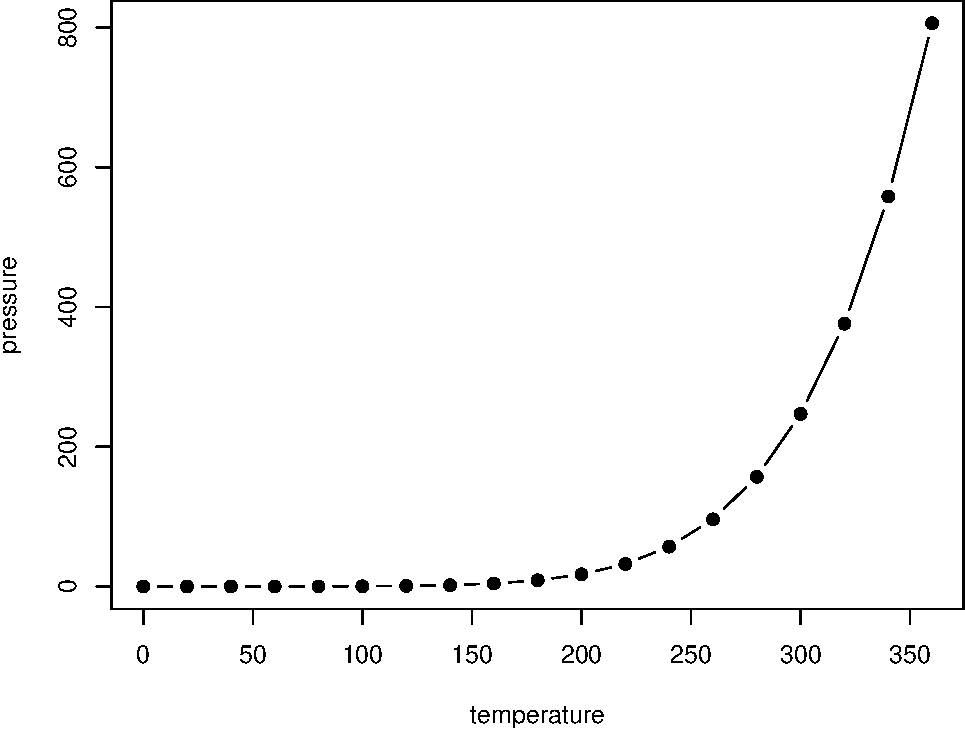
\includegraphics[width=0.8\linewidth]{01-intro_files/figure-latex/nice-fig-1} 

}

\caption{Here is a nice figure!}\label{fig:nice-fig}
\end{figure}

Reference a figure by its code chunk label with the \texttt{fig:}
prefix, e.g., see Figure \ref{fig:nice-fig}. Similarly, you can
reference tables generated from \texttt{knitr::kable()}, e.g., see Table
\ref{tab:nice-tab}.

\begin{Shaded}
\begin{Highlighting}[]
\NormalTok{knitr::}\KeywordTok{kable}\NormalTok{(}
  \KeywordTok{head}\NormalTok{(iris, }\DecValTok{20}\NormalTok{), }\DataTypeTok{caption =} \StringTok{'Here is a nice table!'}\NormalTok{,}
  \DataTypeTok{booktabs =} \OtherTok{TRUE}
\NormalTok{)}
\end{Highlighting}
\end{Shaded}

\begin{table}

\caption{\label{tab:nice-tab}Here is a nice table!}
\centering
\begin{tabular}[t]{rrrrl}
\toprule
Sepal.Length & Sepal.Width & Petal.Length & Petal.Width & Species\\
\midrule
5.1 & 3.5 & 1.4 & 0.2 & setosa\\
4.9 & 3.0 & 1.4 & 0.2 & setosa\\
4.7 & 3.2 & 1.3 & 0.2 & setosa\\
4.6 & 3.1 & 1.5 & 0.2 & setosa\\
5.0 & 3.6 & 1.4 & 0.2 & setosa\\
\addlinespace
5.4 & 3.9 & 1.7 & 0.4 & setosa\\
4.6 & 3.4 & 1.4 & 0.3 & setosa\\
5.0 & 3.4 & 1.5 & 0.2 & setosa\\
4.4 & 2.9 & 1.4 & 0.2 & setosa\\
4.9 & 3.1 & 1.5 & 0.1 & setosa\\
\addlinespace
5.4 & 3.7 & 1.5 & 0.2 & setosa\\
4.8 & 3.4 & 1.6 & 0.2 & setosa\\
4.8 & 3.0 & 1.4 & 0.1 & setosa\\
4.3 & 3.0 & 1.1 & 0.1 & setosa\\
5.8 & 4.0 & 1.2 & 0.2 & setosa\\
\addlinespace
5.7 & 4.4 & 1.5 & 0.4 & setosa\\
5.4 & 3.9 & 1.3 & 0.4 & setosa\\
5.1 & 3.5 & 1.4 & 0.3 & setosa\\
5.7 & 3.8 & 1.7 & 0.3 & setosa\\
5.1 & 3.8 & 1.5 & 0.3 & setosa\\
\bottomrule
\end{tabular}
\end{table}

\chapter{Linear models and matrix algebra}\label{linear-models}

\section{Exercises}\label{exercises}

Solutions to exercises can be found in appendix
\ref{solutions-linear-models}

\chapter{Linear and non linear logistic
regression}\label{logistic-regression}

\section{Exercises}\label{exercises-1}

Solutions to exercises can be found in appendix
\ref{solutions-logistic-regression}.

\chapter{Nearest neighbours}\label{nearest-neighbours}

\section{Example one}\label{example-one}

\section{Example two}\label{example-two}

\section{Exercises}\label{exercises-2}

Solutions to exercises can be found in appendix
\ref{solutions-nearest-neighbours}.

\chapter{Decision trees and random forests}\label{decision-trees}

\section{Exercises}\label{exercises-3}

Solutions to exercises can be found in appendix
\ref{solutions-decision-trees}.

\chapter{Support vector machines}\label{svm}

\section{Exercises}\label{exercises-4}

Solutions to exercises can be found in appendix \ref{solutions-svm}

\chapter{Artificial neural networks}\label{ann}

\section{Exercises}\label{exercises-5}

Solutions to exercises can be found in appendix \ref{solutions-ann}.

\chapter{Dimensionality reduction}\label{dimensionality-reduction}

\section{Linear Dimensionality
Reduction}\label{linear-dimensionality-reduction}

\subsection{Principle Component
Analysis}\label{principle-component-analysis}

\subsection{Horeshoe effect}\label{horeshoe-effect}

\section{Nonlinear Dimensionality
Reduction}\label{nonlinear-dimensionality-reduction}

\subsection{t-SNE}\label{t-sne}

\subsection{Gaussian Process Latent Variable
Models}\label{gaussian-process-latent-variable-models}

\subsection{GPLVMs with informative
priors}\label{gplvms-with-informative-priors}

\section{Exercises}\label{exercises-6}

Solutions to exercises can be found in appendix
\ref{solutions-dimensionality-reduction}.

\chapter{Clustering}\label{clustering}

\section{Introduction}\label{introduction}

Hierarchic (produce dendrogram) vs partitioning methods

\begin{figure}

{\centering 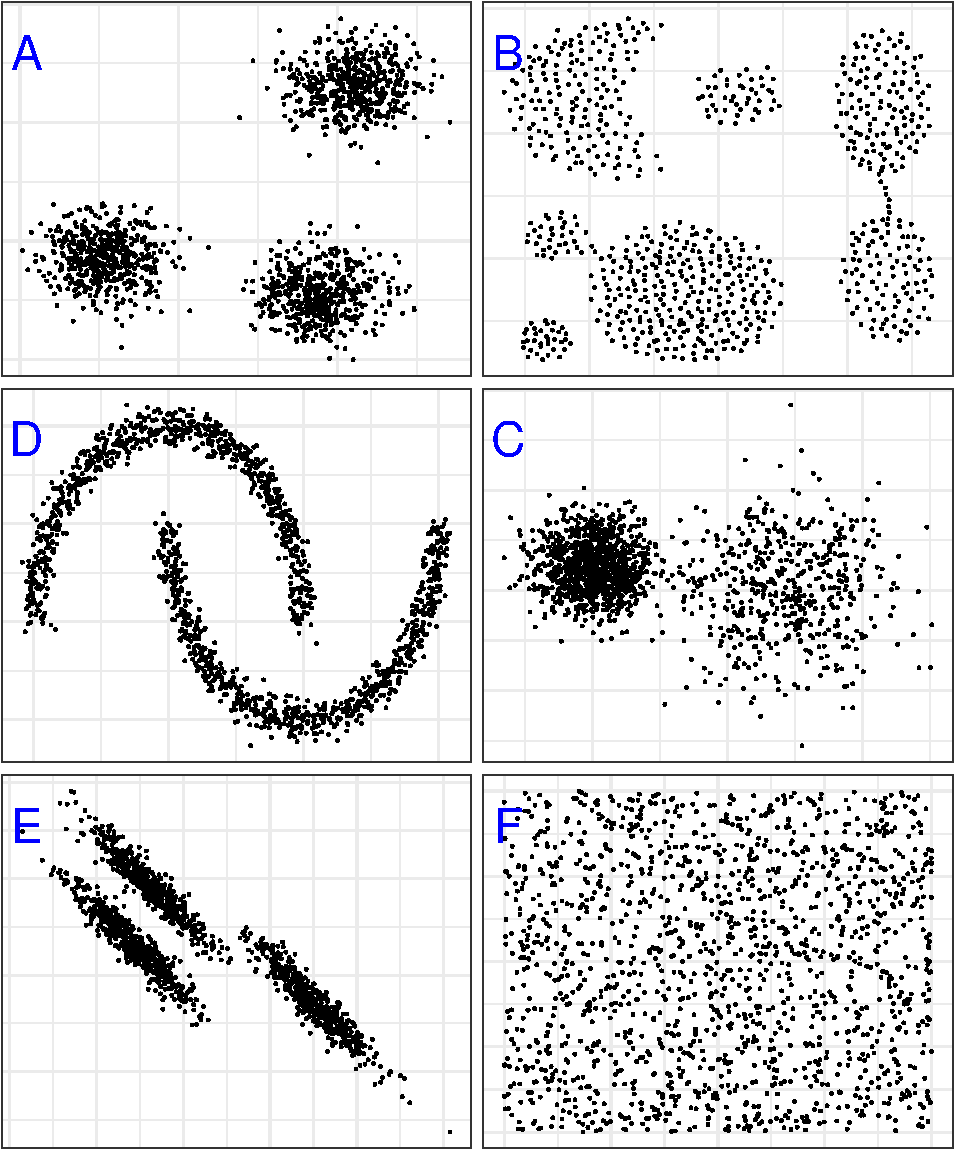
\includegraphics[width=0.8\linewidth]{09-clustering_files/figure-latex/clusterTypes-1} 

}

\caption{Example clusters. **A**, *blobs*; **B**, *aggregation* [@Gionis2007]; **C**, *noisy moons*; **D**, *noisy circles*; **E**, *D31* [@Veenman2002]; **F**, *no structure*.}\label{fig:clusterTypes}
\end{figure}

\section{Distance metrics}\label{distance-metrics}

\textbf{Minkowski distance:}

\begin{equation}
  distance\left(x,y,p\right)=\left(\sum_{i=1}^{n} abs(x_i-y_i)^p\right)^{1/p}
  \label{eq:minkowski}
\end{equation}

Graphical explanation of euclidean, manhattan and max (Chebyshev?)

\subsection{Image segmentation}\label{image-segmentation}

\section{Hierarchic methods}\label{hierarchic-methods}

\begin{table}

\caption{\label{tab:distance-matrix}Example distance matrix}
\centering
\begin{tabular}[t]{lllll}
\toprule
  & A & B & C & D\\
\midrule
B & 2 &  &  & \\
C & 6 & 5 &  & \\
D & 10 & 10 & 5 & \\
E & 9 & 8 & 3 & 4\\
\bottomrule
\end{tabular}
\end{table}

\subsection{Linkage algorithms}\label{linkage-algorithms}

Make one section panel of three dendrograms one table

Single linkage - nearest neighbours linkage Complete linkage - furthest
neighbours linkage Average linkage - UPGMA (Unweighted Pair Group Method
with Arithmetic Mean)

\begin{table}

\caption{\label{tab:distance-merge}Merge distances for objects in the example distance matrix using three different linkage methods.}
\centering
\begin{tabular}[t]{llll}
\toprule
Groups & Single & Complete & Average\\
\midrule
A,B,C,D,E & 0 & 0 & 0\\
(A,B),C,D,E & 2 & 2 & 2\\
(A,B),(C,E),D & 3 & 3 & 3\\
(A,B)(C,D,E) & 4 & 5 & 4.5\\
(A,B,C,D,E) & 5 & 10 & 8\\
\bottomrule
\end{tabular}
\end{table}

\begin{figure}

{\centering 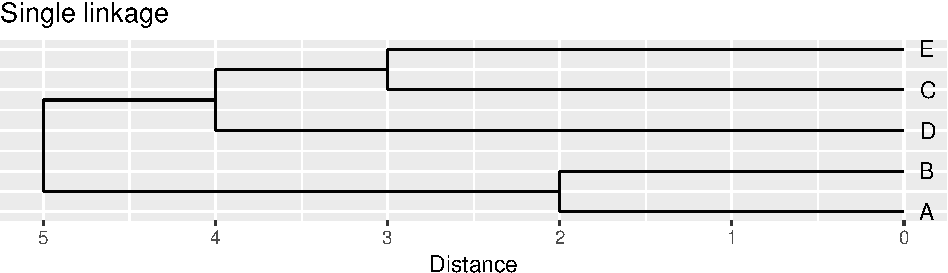
\includegraphics[width=1\linewidth]{09-clustering_files/figure-latex/linkageComparison-1} 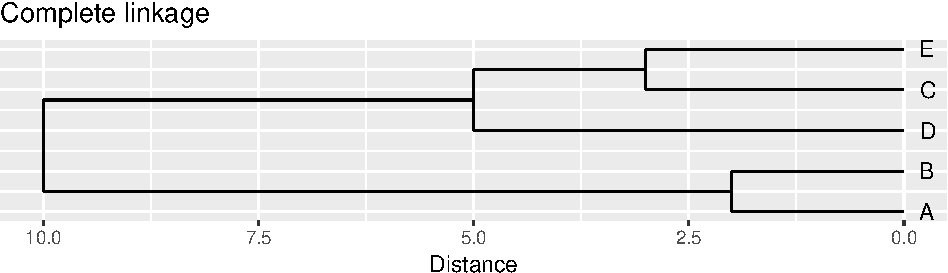
\includegraphics[width=1\linewidth]{09-clustering_files/figure-latex/linkageComparison-2} 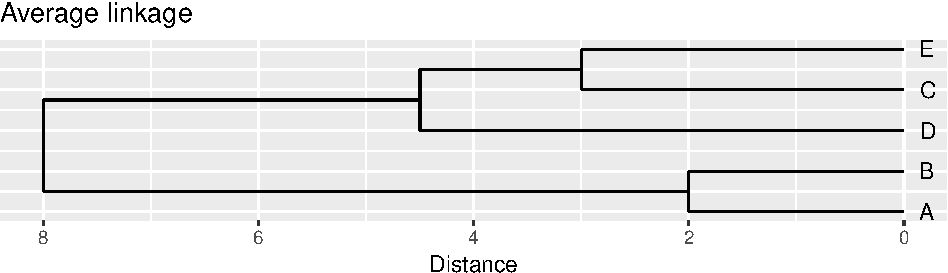
\includegraphics[width=1\linewidth]{09-clustering_files/figure-latex/linkageComparison-3} 

}

\caption{Dendrograms for the example distance matrix using three different linkage methods. }\label{fig:linkageComparison}
\end{figure}

\subsection{Example: clustering toy data
sets}\label{example-clustering-toy-data-sets}

\begin{Shaded}
\begin{Highlighting}[]
\KeywordTok{library}\NormalTok{(RColorBrewer)}
\KeywordTok{library}\NormalTok{(dendextend)}
\end{Highlighting}
\end{Shaded}

\begin{verbatim}
## 
## ---------------------
## Welcome to dendextend version 1.5.2
## Type citation('dendextend') for how to cite the package.
## 
## Type browseVignettes(package = 'dendextend') for the package vignette.
## The github page is: https://github.com/talgalili/dendextend/
## 
## Suggestions and bug-reports can be submitted at: https://github.com/talgalili/dendextend/issues
## Or contact: <tal.galili@gmail.com>
## 
##  To suppress this message use:  suppressPackageStartupMessages(library(dendextend))
## ---------------------
\end{verbatim}

\begin{verbatim}
## 
## Attaching package: 'dendextend'
\end{verbatim}

\begin{verbatim}
## The following object is masked from 'package:ggdendro':
## 
##     theme_dendro
\end{verbatim}

\begin{verbatim}
## The following object is masked from 'package:stats':
## 
##     cutree
\end{verbatim}

\begin{Shaded}
\begin{Highlighting}[]
\KeywordTok{library}\NormalTok{(ggplot2)}
\KeywordTok{library}\NormalTok{(GGally)}

\NormalTok{cluster_colours <-}\StringTok{ }\KeywordTok{brewer.pal}\NormalTok{(}\DecValTok{8}\NormalTok{,}\StringTok{"Dark2"}\NormalTok{)}

\NormalTok{blobs <-}\StringTok{ }\KeywordTok{read.csv}\NormalTok{(}\StringTok{"data/example_clusters/blobs.csv"}\NormalTok{, }\DataTypeTok{header=}\NormalTok{F)}
\end{Highlighting}
\end{Shaded}

\begin{Shaded}
\begin{Highlighting}[]
\NormalTok{aggregation <-}\StringTok{ }\KeywordTok{read.table}\NormalTok{(}\StringTok{"data/example_clusters/aggregation.txt"}\NormalTok{)}
\NormalTok{noisy_moons <-}\StringTok{ }\KeywordTok{read.csv}\NormalTok{(}\StringTok{"data/example_clusters/noisy_moons.csv"}\NormalTok{, }\DataTypeTok{header=}\NormalTok{F)}
\NormalTok{noisy_circles <-}\StringTok{ }\KeywordTok{read.csv}\NormalTok{(}\StringTok{"data/example_clusters/noisy_circles.csv"}\NormalTok{, }\DataTypeTok{header=}\NormalTok{F)}
\NormalTok{no_structure <-}\StringTok{ }\KeywordTok{read.csv}\NormalTok{(}\StringTok{"data/example_clusters/no_structure.csv"}\NormalTok{, }\DataTypeTok{header=}\NormalTok{F)}

\NormalTok{hclust_plots <-}\StringTok{ }\NormalTok{function(data_set, n)\{}
  \NormalTok{d <-}\StringTok{ }\KeywordTok{dist}\NormalTok{(data_set[,}\DecValTok{1}\NormalTok{:}\DecValTok{2}\NormalTok{])}
  \NormalTok{dend <-}\StringTok{ }\KeywordTok{as.dendrogram}\NormalTok{(}\KeywordTok{hclust}\NormalTok{(d, }\DataTypeTok{method=}\StringTok{"average"}\NormalTok{))}
  \NormalTok{clusters <-}\StringTok{ }\KeywordTok{cutree}\NormalTok{(dend,n,}\DataTypeTok{order_clusters_as_data=}\NormalTok{F)}
  \NormalTok{dend <-}\StringTok{ }\KeywordTok{color_branches}\NormalTok{(dend, }\DataTypeTok{clusters=}\NormalTok{clusters, }\DataTypeTok{col=}\NormalTok{cluster_colours[}\DecValTok{1}\NormalTok{:n])}
  \NormalTok{clusters <-}\StringTok{ }\NormalTok{clusters[}\KeywordTok{order}\NormalTok{(}\KeywordTok{as.numeric}\NormalTok{(}\KeywordTok{names}\NormalTok{(clusters)))]}
  \KeywordTok{labels}\NormalTok{(dend) <-}\StringTok{ }\KeywordTok{rep}\NormalTok{(}\StringTok{""}\NormalTok{, }\KeywordTok{length}\NormalTok{(data_set[,}\DecValTok{1}\NormalTok{]))}
  \NormalTok{ggd <-}\StringTok{ }\KeywordTok{as.ggdend}\NormalTok{(dend)}
  \NormalTok{ggd$nodes <-}\StringTok{ }\NormalTok{ggd$nodes[!(}\DecValTok{1}\NormalTok{:}\KeywordTok{length}\NormalTok{(ggd$nodes[,}\DecValTok{1}\NormalTok{])),]}
  \NormalTok{plotPair <-}\StringTok{ }\KeywordTok{list}\NormalTok{(}\KeywordTok{ggplot}\NormalTok{(ggd),}
    \KeywordTok{ggplot}\NormalTok{(data_set, }\KeywordTok{aes}\NormalTok{(V1,V2)) +}\StringTok{ }\KeywordTok{geom_point}\NormalTok{(}\DataTypeTok{col=}\NormalTok{cluster_colours[clusters], }\DataTypeTok{size=}\FloatTok{0.2}\NormalTok{))}
  \KeywordTok{return}\NormalTok{(plotPair)}
\NormalTok{\}}

\NormalTok{plotList <-}\StringTok{ }\KeywordTok{c}\NormalTok{(}
  \KeywordTok{hclust_plots}\NormalTok{(aggregation, }\DecValTok{7}\NormalTok{),}
  \KeywordTok{hclust_plots}\NormalTok{(noisy_moons, }\DecValTok{2}\NormalTok{),}
  \KeywordTok{hclust_plots}\NormalTok{(noisy_circles, }\DecValTok{2}\NormalTok{),}
  \KeywordTok{hclust_plots}\NormalTok{(no_structure, }\DecValTok{3}\NormalTok{)}
\NormalTok{)}

\NormalTok{pm <-}\StringTok{ }\KeywordTok{ggmatrix}\NormalTok{(}
  \NormalTok{plotList, }\DataTypeTok{nrow=}\DecValTok{4}\NormalTok{, }\DataTypeTok{ncol=}\DecValTok{2}\NormalTok{, }\DataTypeTok{showXAxisPlotLabels =} \NormalTok{F, }\DataTypeTok{showYAxisPlotLabels =} \NormalTok{F, }\DataTypeTok{xAxisLabels=}\KeywordTok{c}\NormalTok{(}\StringTok{"dendrogram"}\NormalTok{, }\StringTok{"scatter plot"}\NormalTok{), }\DataTypeTok{yAxisLabels=}\KeywordTok{c}\NormalTok{(}\StringTok{"aggregation"}\NormalTok{, }\StringTok{"noisy moons"}\NormalTok{, }\StringTok{"noisy circles"}\NormalTok{, }\StringTok{"no structure"}\NormalTok{)}
\NormalTok{) +}\StringTok{ }\KeywordTok{theme_bw}\NormalTok{()}

\NormalTok{pm}
\end{Highlighting}
\end{Shaded}

\begin{figure}

{\centering 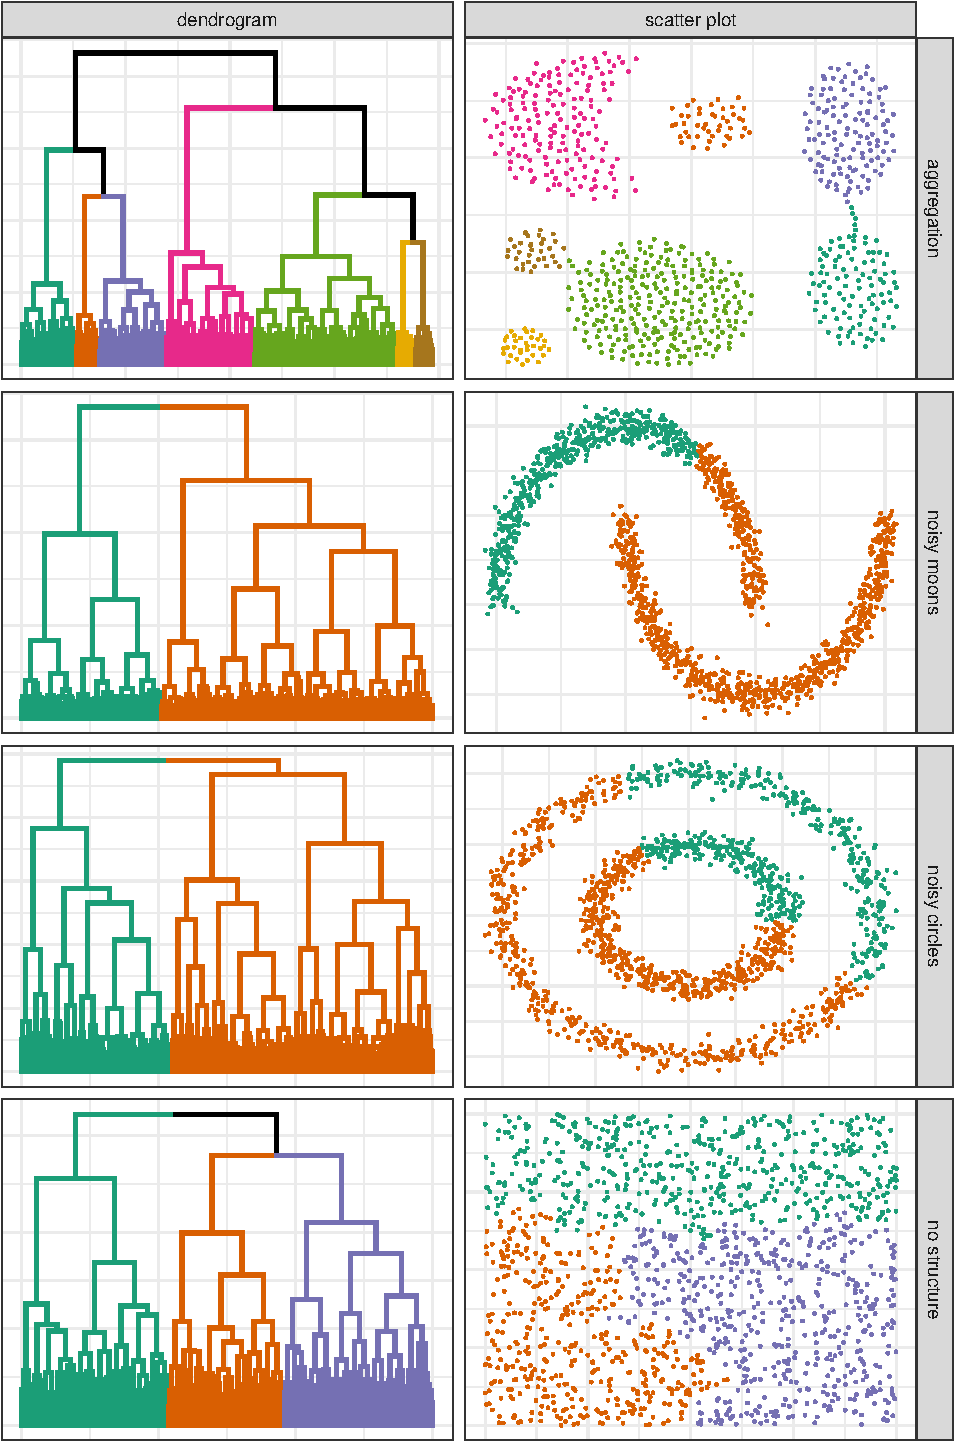
\includegraphics[width=0.75\linewidth]{09-clustering_files/figure-latex/hclustToyData-1} 

}

\caption{Hierarchical clustering of toy data-sets. }\label{fig:hclustToyData}
\end{figure}

\subsection{Example: gene expression profiling of human
tissues}\label{example-gene-expression-profiling-of-human-tissues}

Load required libraries

\begin{Shaded}
\begin{Highlighting}[]
\KeywordTok{library}\NormalTok{(RColorBrewer)}
\KeywordTok{library}\NormalTok{(dendextend)}
\end{Highlighting}
\end{Shaded}

Load data

\begin{Shaded}
\begin{Highlighting}[]
\KeywordTok{load}\NormalTok{(}\StringTok{"data/tissues_gene_expression/tissuesGeneExpression.rda"}\NormalTok{)}
\end{Highlighting}
\end{Shaded}

Inspect data

\begin{Shaded}
\begin{Highlighting}[]
\KeywordTok{table}\NormalTok{(tissue)}
\end{Highlighting}
\end{Shaded}

\begin{verbatim}
## tissue
##  cerebellum       colon endometrium hippocampus      kidney       liver 
##          38          34          15          31          39          26 
##    placenta 
##           6
\end{verbatim}

\begin{Shaded}
\begin{Highlighting}[]
\KeywordTok{dim}\NormalTok{(e)}
\end{Highlighting}
\end{Shaded}

\begin{verbatim}
## [1] 22215   189
\end{verbatim}

Compute distance between each sample

\begin{Shaded}
\begin{Highlighting}[]
\NormalTok{d <-}\StringTok{ }\KeywordTok{dist}\NormalTok{(}\KeywordTok{t}\NormalTok{(e))}
\end{Highlighting}
\end{Shaded}

perform hierarchical clustering

\begin{Shaded}
\begin{Highlighting}[]
\NormalTok{hc <-}\StringTok{ }\KeywordTok{hclust}\NormalTok{(d, }\DataTypeTok{method=}\StringTok{"average"}\NormalTok{)}
\KeywordTok{plot}\NormalTok{(hc, }\DataTypeTok{labels=}\NormalTok{tissue, }\DataTypeTok{cex=}\FloatTok{0.5}\NormalTok{, }\DataTypeTok{hang=}\NormalTok{-}\DecValTok{1}\NormalTok{, }\DataTypeTok{xlab=}\StringTok{""}\NormalTok{, }\DataTypeTok{sub=}\StringTok{""}\NormalTok{)}
\end{Highlighting}
\end{Shaded}

\begin{figure}

{\centering 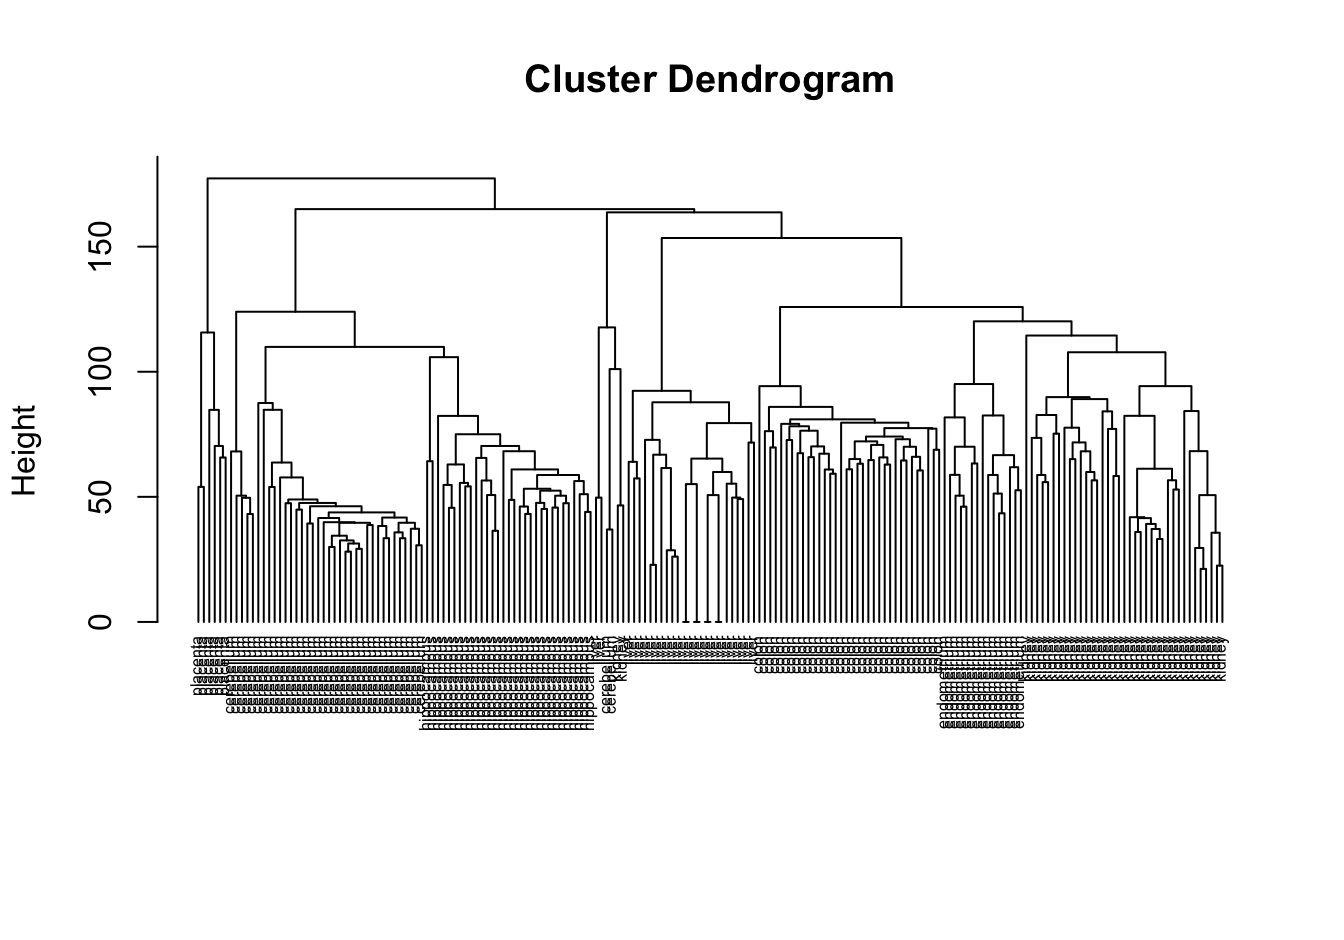
\includegraphics[width=1\linewidth]{09-clustering_files/figure-latex/tissueDendrogram-1} 

}

\caption{Clustering of tissue samples based on gene expression profiles. }\label{fig:tissueDendrogram}
\end{figure}

use dendextend library to plot dendrogram with colour labels

\begin{Shaded}
\begin{Highlighting}[]
\NormalTok{tissue_type <-}\StringTok{ }\KeywordTok{unique}\NormalTok{(tissue)}
\NormalTok{dend <-}\StringTok{ }\KeywordTok{as.dendrogram}\NormalTok{(hc)}
\NormalTok{dend_colours <-}\StringTok{ }\KeywordTok{brewer.pal}\NormalTok{(}\KeywordTok{length}\NormalTok{(}\KeywordTok{unique}\NormalTok{(tissue)),}\StringTok{"Dark2"}\NormalTok{)}
\KeywordTok{names}\NormalTok{(dend_colours) <-}\StringTok{ }\NormalTok{tissue_type}
\KeywordTok{labels}\NormalTok{(dend) <-}\StringTok{ }\NormalTok{tissue[}\KeywordTok{order.dendrogram}\NormalTok{(dend)]}
\KeywordTok{labels_colors}\NormalTok{(dend) <-}\StringTok{ }\NormalTok{dend_colours[tissue][}\KeywordTok{order.dendrogram}\NormalTok{(dend)]}
\KeywordTok{labels_cex}\NormalTok{(dend) =}\StringTok{ }\FloatTok{0.5}
\KeywordTok{plot}\NormalTok{(dend, }\DataTypeTok{horiz=}\NormalTok{T)}
\end{Highlighting}
\end{Shaded}

\begin{figure}

{\centering 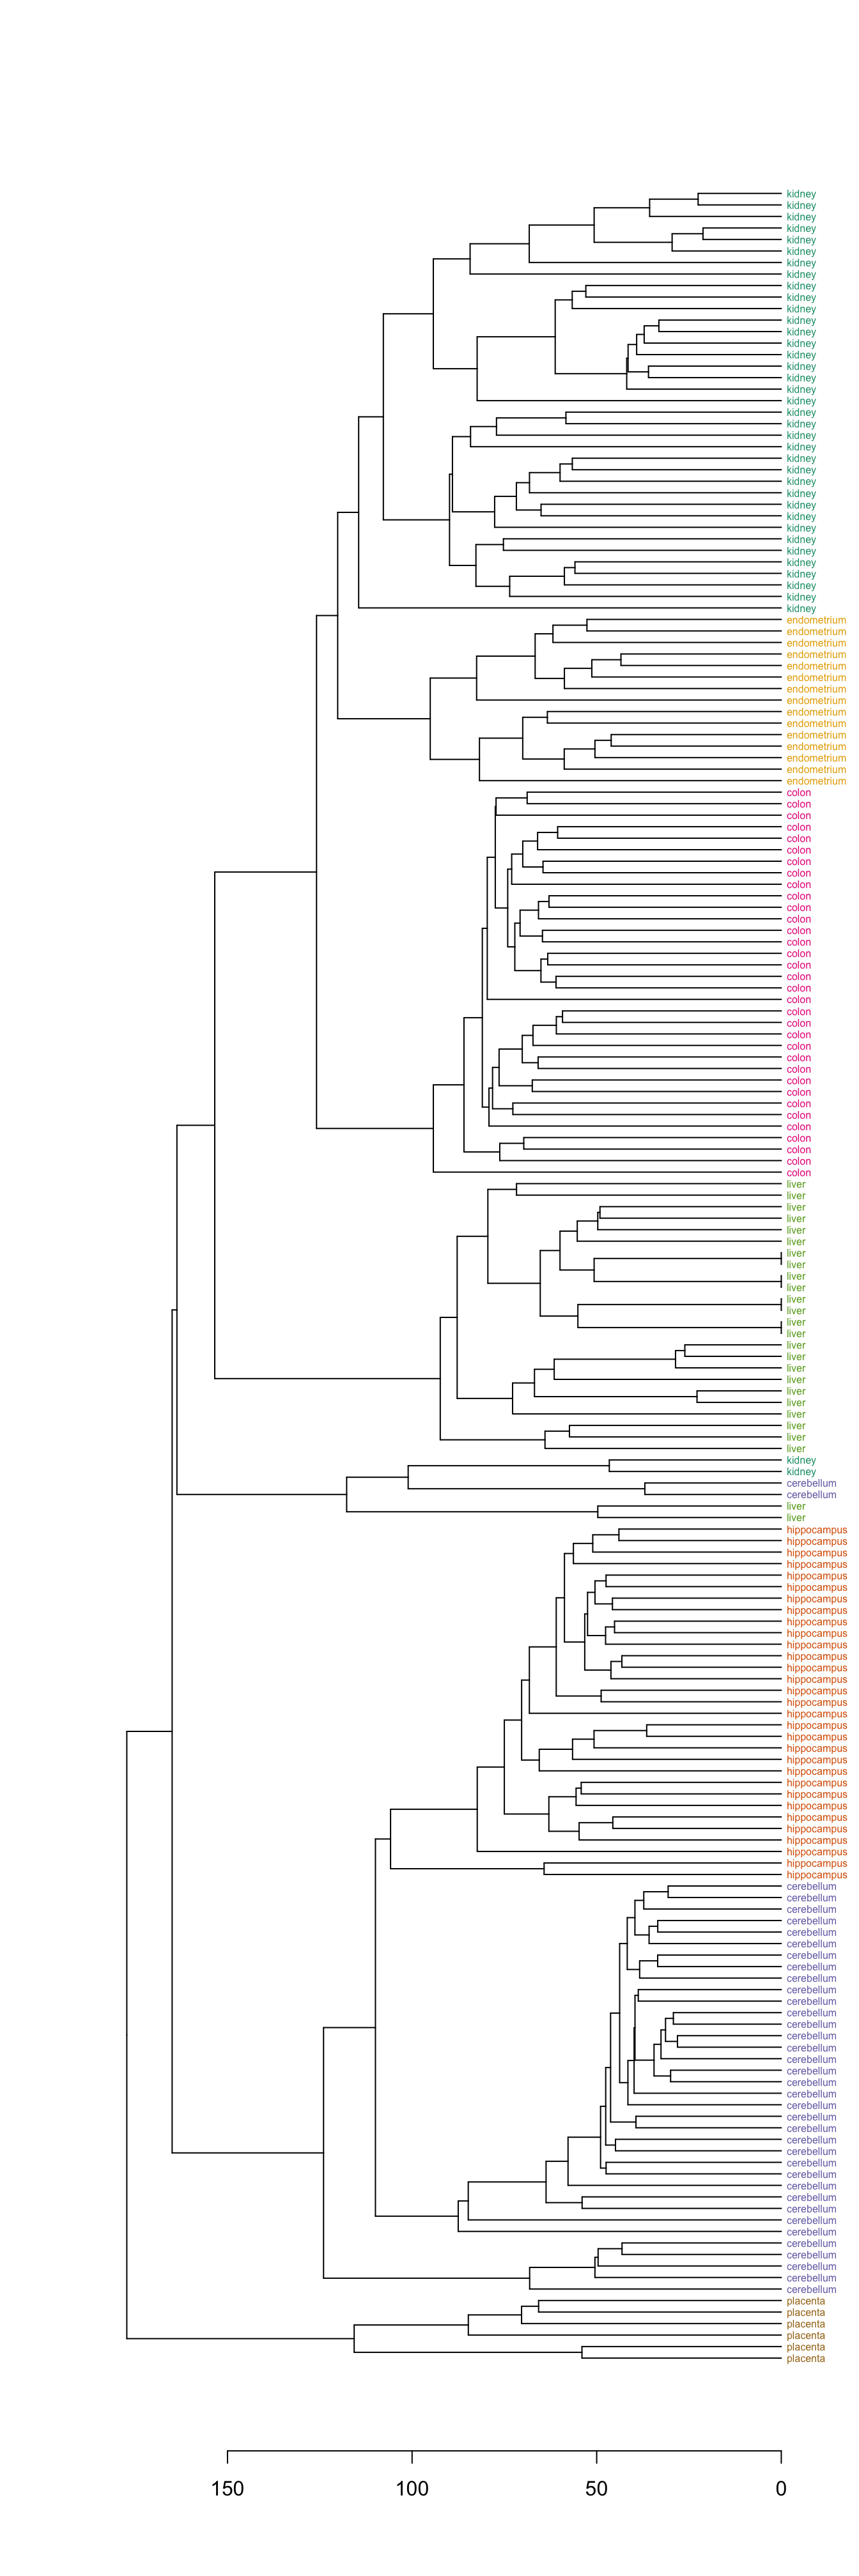
\includegraphics[width=1\linewidth]{09-clustering_files/figure-latex/tissueDendrogramColour-1} 

}

\caption{Clustering of tissue samples based on gene expression profiles with labels coloured by tissue type. }\label{fig:tissueDendrogramColour}
\end{figure}

Define clusters by cutting tree at a specific height

\begin{Shaded}
\begin{Highlighting}[]
\KeywordTok{plot}\NormalTok{(dend, }\DataTypeTok{horiz=}\NormalTok{T)}
\KeywordTok{abline}\NormalTok{(}\DataTypeTok{v=}\DecValTok{125}\NormalTok{, }\DataTypeTok{lwd=}\DecValTok{2}\NormalTok{, }\DataTypeTok{lty=}\DecValTok{2}\NormalTok{, }\DataTypeTok{col=}\StringTok{"blue"}\NormalTok{)}
\end{Highlighting}
\end{Shaded}

\begin{figure}

{\centering 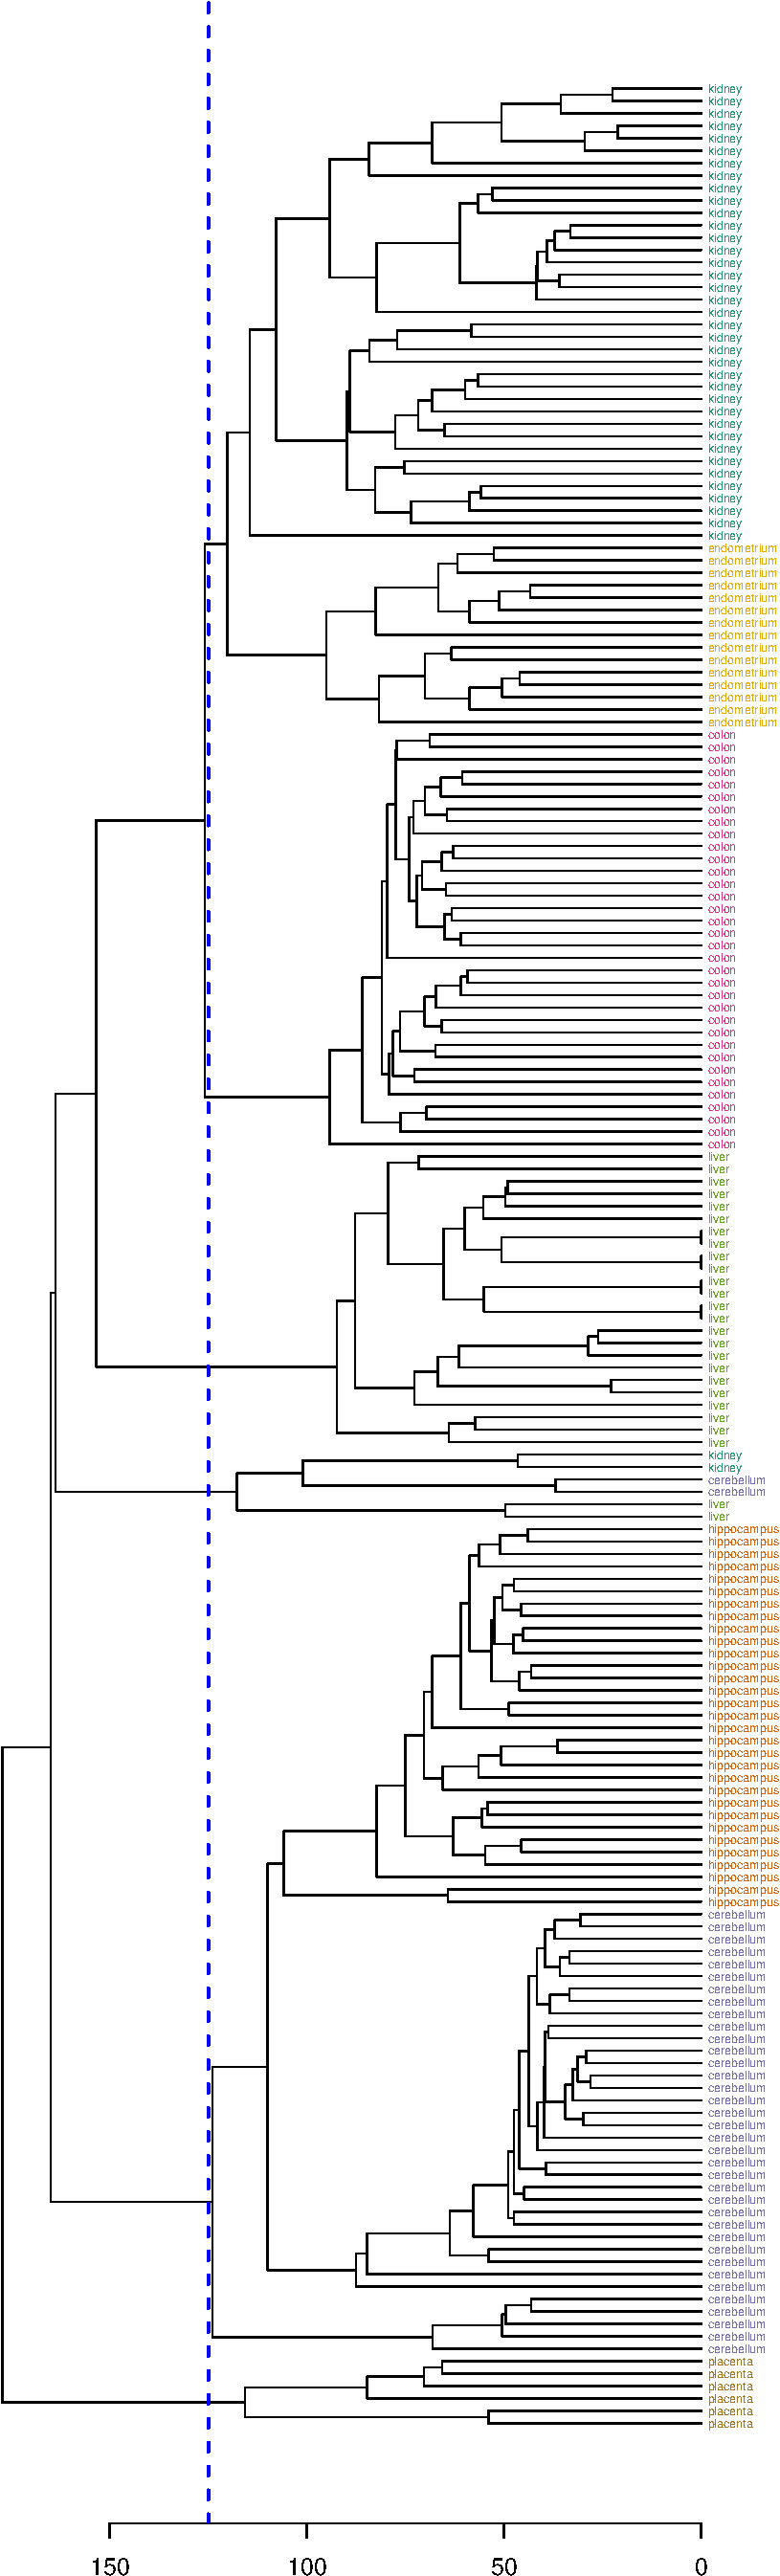
\includegraphics[width=1\linewidth]{09-clustering_files/figure-latex/tissueDendrogramCutHeight-1} 

}

\caption{Clusters found by cutting tree at a height of 125}\label{fig:tissueDendrogramCutHeight}
\end{figure}

\begin{Shaded}
\begin{Highlighting}[]
\NormalTok{hclusters <-}\StringTok{ }\KeywordTok{cutree}\NormalTok{(dend, }\DataTypeTok{h=}\DecValTok{125}\NormalTok{)}
\KeywordTok{table}\NormalTok{(tissue, }\DataTypeTok{cluster=}\NormalTok{hclusters)}
\end{Highlighting}
\end{Shaded}

\begin{verbatim}
##              cluster
## tissue         1  2  3  4  5  6
##   cerebellum   0 36  0  0  2  0
##   colon        0  0 34  0  0  0
##   endometrium 15  0  0  0  0  0
##   hippocampus  0 31  0  0  0  0
##   kidney      37  0  0  0  2  0
##   liver        0  0  0 24  2  0
##   placenta     0  0  0  0  0  6
\end{verbatim}

Select a specific number of clusters.

\begin{Shaded}
\begin{Highlighting}[]
\KeywordTok{plot}\NormalTok{(dend, }\DataTypeTok{horiz=}\NormalTok{T)}
\KeywordTok{abline}\NormalTok{(}\DataTypeTok{v =} \KeywordTok{heights_per_k.dendrogram}\NormalTok{(dend)[}\StringTok{"8"}\NormalTok{], }\DataTypeTok{lwd =} \DecValTok{2}\NormalTok{, }\DataTypeTok{lty =} \DecValTok{2}\NormalTok{, }\DataTypeTok{col =} \StringTok{"blue"}\NormalTok{)}
\end{Highlighting}
\end{Shaded}

\begin{figure}

{\centering 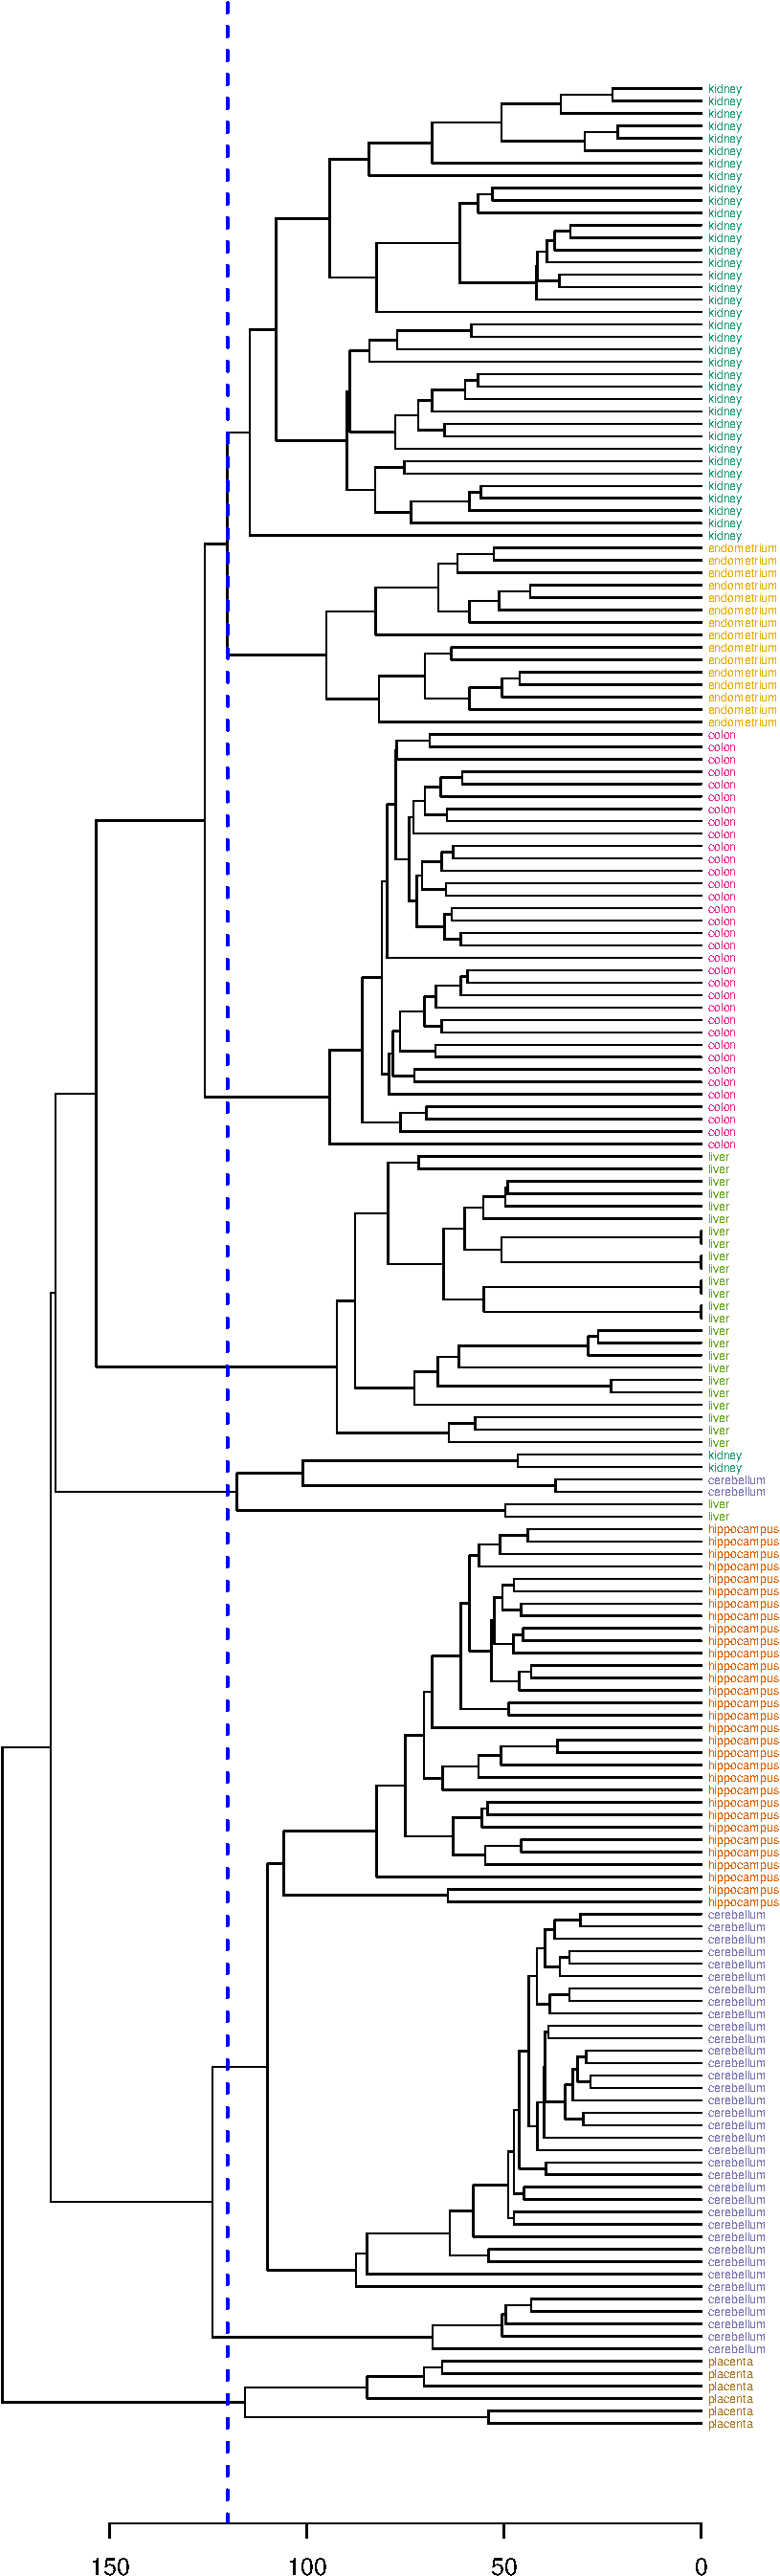
\includegraphics[width=1\linewidth]{09-clustering_files/figure-latex/tissueDendrogramEightClusters-1} 

}

\caption{Selection of eight clusters from the dendogram}\label{fig:tissueDendrogramEightClusters}
\end{figure}

\begin{Shaded}
\begin{Highlighting}[]
\NormalTok{hclusters <-}\StringTok{ }\KeywordTok{cutree}\NormalTok{(dend, }\DataTypeTok{k=}\DecValTok{8}\NormalTok{)}
\KeywordTok{table}\NormalTok{(tissue, }\DataTypeTok{cluster=}\NormalTok{hclusters)}
\end{Highlighting}
\end{Shaded}

\begin{verbatim}
##              cluster
## tissue         1  2  3  4  5  6  7  8
##   cerebellum   0 31  0  0  2  0  5  0
##   colon        0  0 34  0  0  0  0  0
##   endometrium  0  0  0  0  0 15  0  0
##   hippocampus  0 31  0  0  0  0  0  0
##   kidney      37  0  0  0  2  0  0  0
##   liver        0  0  0 24  2  0  0  0
##   placenta     0  0  0  0  0  0  0  6
\end{verbatim}

\section{Partitioning methods}\label{partitioning-methods}

\subsection{K-means}\label{k-means}

\subsubsection{Algorithm}\label{algorithm}

Pseudocode

to illustrate range of different types of data that can be clustered -
image segmentation

\begin{figure}

{\centering 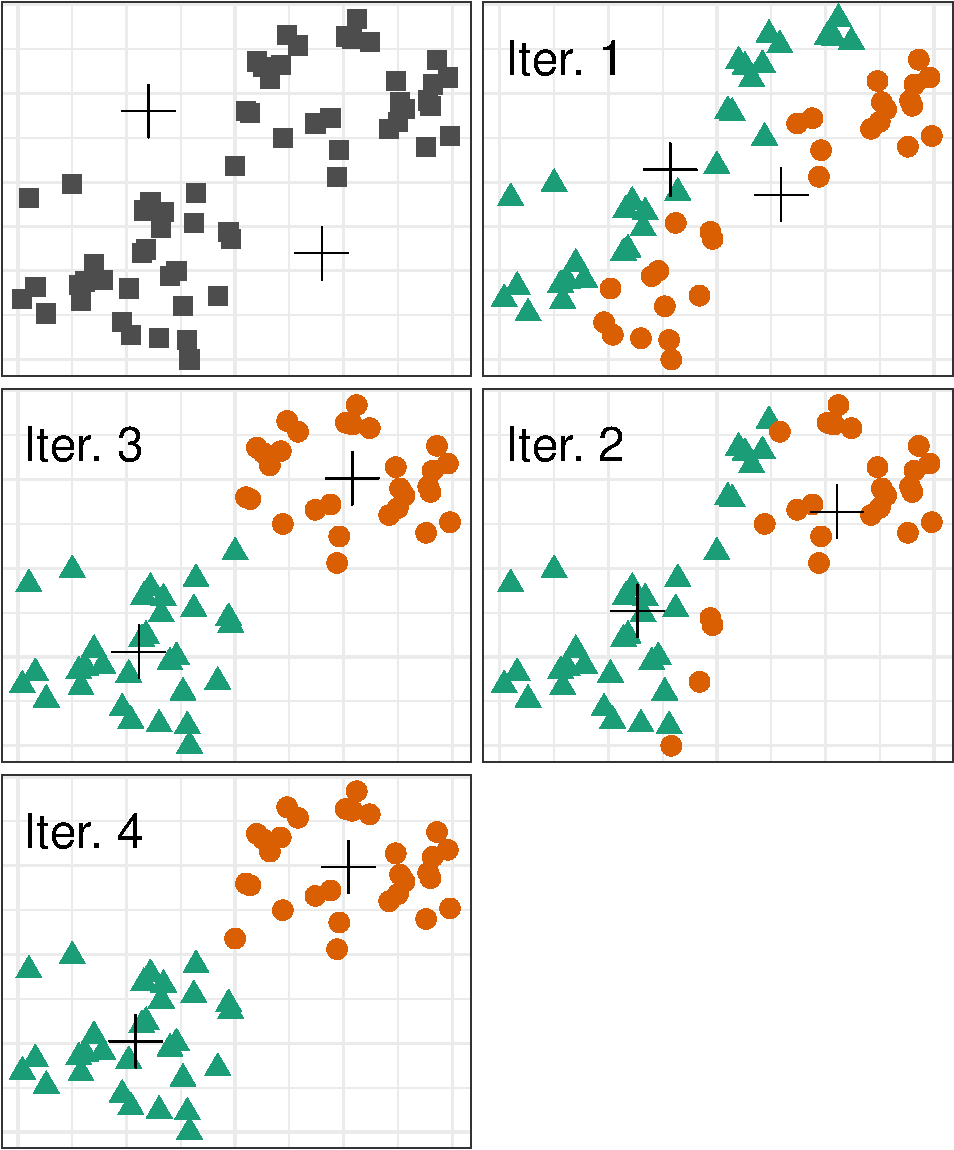
\includegraphics[width=0.9\linewidth]{09-clustering_files/figure-latex/kmeansIterations-1} 

}

\caption{Iterations of the k-means algorithm}\label{fig:kmeansIterations}
\end{figure}

The default setting of the \textbf{kmeans} function is to perform a
maximum of 10 iterations and if the algorithm fails to converge a
warning is issued. The maximum number of iterations is set with the
argument \textbf{iter.max}.

\subsubsection{Choosing initial cluster
centres}\label{choosing-initial-cluster-centres}

\begin{Shaded}
\begin{Highlighting}[]
\KeywordTok{library}\NormalTok{(RColorBrewer)}
\NormalTok{point_shapes <-}\StringTok{ }\KeywordTok{c}\NormalTok{(}\DecValTok{15}\NormalTok{,}\DecValTok{17}\NormalTok{,}\DecValTok{19}\NormalTok{)}
\NormalTok{point_colours <-}\StringTok{ }\KeywordTok{brewer.pal}\NormalTok{(}\DecValTok{3}\NormalTok{,}\StringTok{"Dark2"}\NormalTok{)}
\NormalTok{point_size =}\StringTok{ }\FloatTok{1.5}
\NormalTok{center_point_size =}\StringTok{ }\DecValTok{8}

\NormalTok{blobs <-}\StringTok{ }\KeywordTok{as.data.frame}\NormalTok{(}\KeywordTok{read.csv}\NormalTok{(}\StringTok{"data/example_clusters/blobs.csv"}\NormalTok{, }\DataTypeTok{header=}\NormalTok{F))}

\NormalTok{good_centres <-}\StringTok{ }\KeywordTok{as.data.frame}\NormalTok{(}\KeywordTok{matrix}\NormalTok{(}\KeywordTok{c}\NormalTok{(}\DecValTok{2}\NormalTok{,}\DecValTok{8}\NormalTok{,}\DecValTok{7}\NormalTok{,}\DecValTok{3}\NormalTok{,}\DecValTok{12}\NormalTok{,}\DecValTok{7}\NormalTok{), }\DataTypeTok{ncol=}\DecValTok{2}\NormalTok{, }\DataTypeTok{byrow=}\NormalTok{T))}
\NormalTok{bad_centres <-}\StringTok{ }\KeywordTok{as.data.frame}\NormalTok{(}\KeywordTok{matrix}\NormalTok{(}\KeywordTok{c}\NormalTok{(}\DecValTok{13}\NormalTok{,}\DecValTok{13}\NormalTok{,}\DecValTok{8}\NormalTok{,}\DecValTok{12}\NormalTok{,}\DecValTok{2}\NormalTok{,}\DecValTok{2}\NormalTok{), }\DataTypeTok{ncol=}\DecValTok{2}\NormalTok{, }\DataTypeTok{byrow=}\NormalTok{T))}

\NormalTok{good_result <-}\StringTok{ }\KeywordTok{kmeans}\NormalTok{(blobs[,}\DecValTok{1}\NormalTok{:}\DecValTok{2}\NormalTok{], }\DataTypeTok{centers=}\NormalTok{good_centres)}
\NormalTok{bad_result <-}\StringTok{ }\KeywordTok{kmeans}\NormalTok{(blobs[,}\DecValTok{1}\NormalTok{:}\DecValTok{2}\NormalTok{], }\DataTypeTok{centers=}\NormalTok{bad_centres)}

\NormalTok{plotList <-}\StringTok{ }\KeywordTok{list}\NormalTok{(}
\KeywordTok{ggplot}\NormalTok{(blobs, }\KeywordTok{aes}\NormalTok{(V1,V2)) +}\StringTok{ }\KeywordTok{geom_point}\NormalTok{(}\DataTypeTok{col=}\NormalTok{point_colours[good_result$cluster], }\DataTypeTok{shape=}\NormalTok{point_shapes[good_result$cluster], }\DataTypeTok{size=}\NormalTok{point_size) +}\StringTok{ }\KeywordTok{geom_point}\NormalTok{(}\DataTypeTok{data=}\NormalTok{good_centres, }\KeywordTok{aes}\NormalTok{(V1,V2), }\DataTypeTok{shape=}\DecValTok{3}\NormalTok{, }\DataTypeTok{col=}\StringTok{"black"}\NormalTok{, }\DataTypeTok{size=}\NormalTok{center_point_size) +}\StringTok{ }\KeywordTok{theme_bw}\NormalTok{(),}
\KeywordTok{ggplot}\NormalTok{(blobs, }\KeywordTok{aes}\NormalTok{(V1,V2)) +}\StringTok{ }\KeywordTok{geom_point}\NormalTok{(}\DataTypeTok{col=}\NormalTok{point_colours[bad_result$cluster], }\DataTypeTok{shape=}\NormalTok{point_shapes[bad_result$cluster], }\DataTypeTok{size=}\NormalTok{point_size) +}\StringTok{ }\KeywordTok{geom_point}\NormalTok{(}\DataTypeTok{data=}\NormalTok{bad_centres, }\KeywordTok{aes}\NormalTok{(V1,V2), }\DataTypeTok{shape=}\DecValTok{3}\NormalTok{, }\DataTypeTok{col=}\StringTok{"black"}\NormalTok{, }\DataTypeTok{size=}\NormalTok{center_point_size) +}\StringTok{ }\KeywordTok{theme_bw}\NormalTok{()}
\NormalTok{)}

\NormalTok{pm <-}\StringTok{ }\KeywordTok{ggmatrix}\NormalTok{(}
  \NormalTok{plotList, }\DataTypeTok{nrow=}\DecValTok{1}\NormalTok{, }\DataTypeTok{ncol=}\DecValTok{2}\NormalTok{, }\DataTypeTok{showXAxisPlotLabels =} \NormalTok{T, }\DataTypeTok{showYAxisPlotLabels =} \NormalTok{T, }\DataTypeTok{xAxisLabels=}\KeywordTok{c}\NormalTok{(}\StringTok{"A"}\NormalTok{, }\StringTok{"B"}\NormalTok{)}
\NormalTok{) +}\StringTok{ }\KeywordTok{theme_bw}\NormalTok{()}

\NormalTok{pm}
\end{Highlighting}
\end{Shaded}

\begin{figure}

{\centering 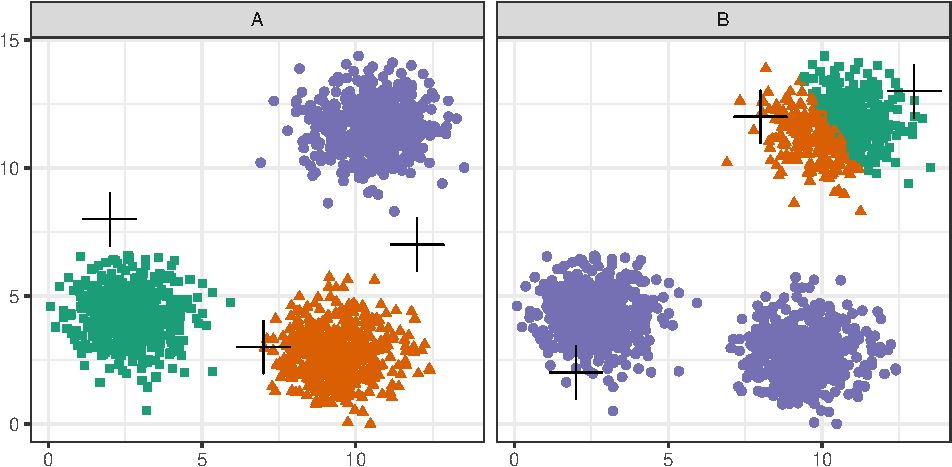
\includegraphics[width=1\linewidth]{09-clustering_files/figure-latex/kmeansCentreChoice-1} 

}

\caption{Initial centres determine clusters. The starting centres are shown as crosses. **A**, real clusters found; **B**, convergence to a local minimum.}\label{fig:kmeansCentreChoice}
\end{figure}

Convergence to a local minimum can be avoided by starting the algorithm
multiple times, with different random centres. The \textbf{nstart}
argument to the \textbf{k-means} function can be used to specify the
number of random sets and optimal solution will be selected
automatically.

\subsubsection{Choosing k}\label{choosing-k}

\begin{Shaded}
\begin{Highlighting}[]
\NormalTok{cluster_colours <-}\StringTok{ }\KeywordTok{brewer.pal}\NormalTok{(}\DecValTok{9}\NormalTok{,}\StringTok{"Set1"}\NormalTok{)}
\NormalTok{k <-}\StringTok{ }\DecValTok{1}\NormalTok{:}\DecValTok{9}
\NormalTok{res <-}\StringTok{ }\KeywordTok{lapply}\NormalTok{(k, function(i)\{}\KeywordTok{kmeans}\NormalTok{(blobs[,}\DecValTok{1}\NormalTok{:}\DecValTok{2}\NormalTok{], i, }\DataTypeTok{nstart=}\DecValTok{50}\NormalTok{)\})}

\NormalTok{plotList <-}\StringTok{ }\KeywordTok{lapply}\NormalTok{(k, function(i)\{}
  \KeywordTok{ggplot}\NormalTok{(blobs, }\KeywordTok{aes}\NormalTok{(V1, V2)) +}\StringTok{ }
\StringTok{    }\KeywordTok{geom_point}\NormalTok{(}\DataTypeTok{col=}\NormalTok{cluster_colours[res[[i]]$cluster], }\DataTypeTok{size=}\DecValTok{1}\NormalTok{) +}
\StringTok{    }\KeywordTok{geom_point}\NormalTok{(}\DataTypeTok{data=}\KeywordTok{as.data.frame}\NormalTok{(res[[i]]$centers), }\KeywordTok{aes}\NormalTok{(V1,V2), }\DataTypeTok{shape=}\DecValTok{3}\NormalTok{, }\DataTypeTok{col=}\StringTok{"black"}\NormalTok{, }\DataTypeTok{size=}\DecValTok{5}\NormalTok{) +}
\StringTok{    }\KeywordTok{annotate}\NormalTok{(}\StringTok{"text"}\NormalTok{, }\DataTypeTok{x=}\DecValTok{2}\NormalTok{, }\DataTypeTok{y=}\DecValTok{13}\NormalTok{, }\DataTypeTok{label=}\KeywordTok{paste}\NormalTok{(}\StringTok{"k="}\NormalTok{, i, }\DataTypeTok{sep=}\StringTok{""}\NormalTok{), }\DataTypeTok{size=}\DecValTok{8}\NormalTok{, }\DataTypeTok{col=}\StringTok{"black"}\NormalTok{) +}
\StringTok{    }\KeywordTok{theme_bw}\NormalTok{()}
\NormalTok{\}}
\NormalTok{)}

\NormalTok{pm <-}\StringTok{ }\KeywordTok{ggmatrix}\NormalTok{(}
  \NormalTok{plotList, }\DataTypeTok{nrow=}\DecValTok{3}\NormalTok{, }\DataTypeTok{ncol=}\DecValTok{3}\NormalTok{, }\DataTypeTok{showXAxisPlotLabels =} \NormalTok{T, }\DataTypeTok{showYAxisPlotLabels =} \NormalTok{T}
\NormalTok{) +}\StringTok{ }\KeywordTok{theme_bw}\NormalTok{()}

\NormalTok{pm}
\end{Highlighting}
\end{Shaded}

\begin{figure}

{\centering 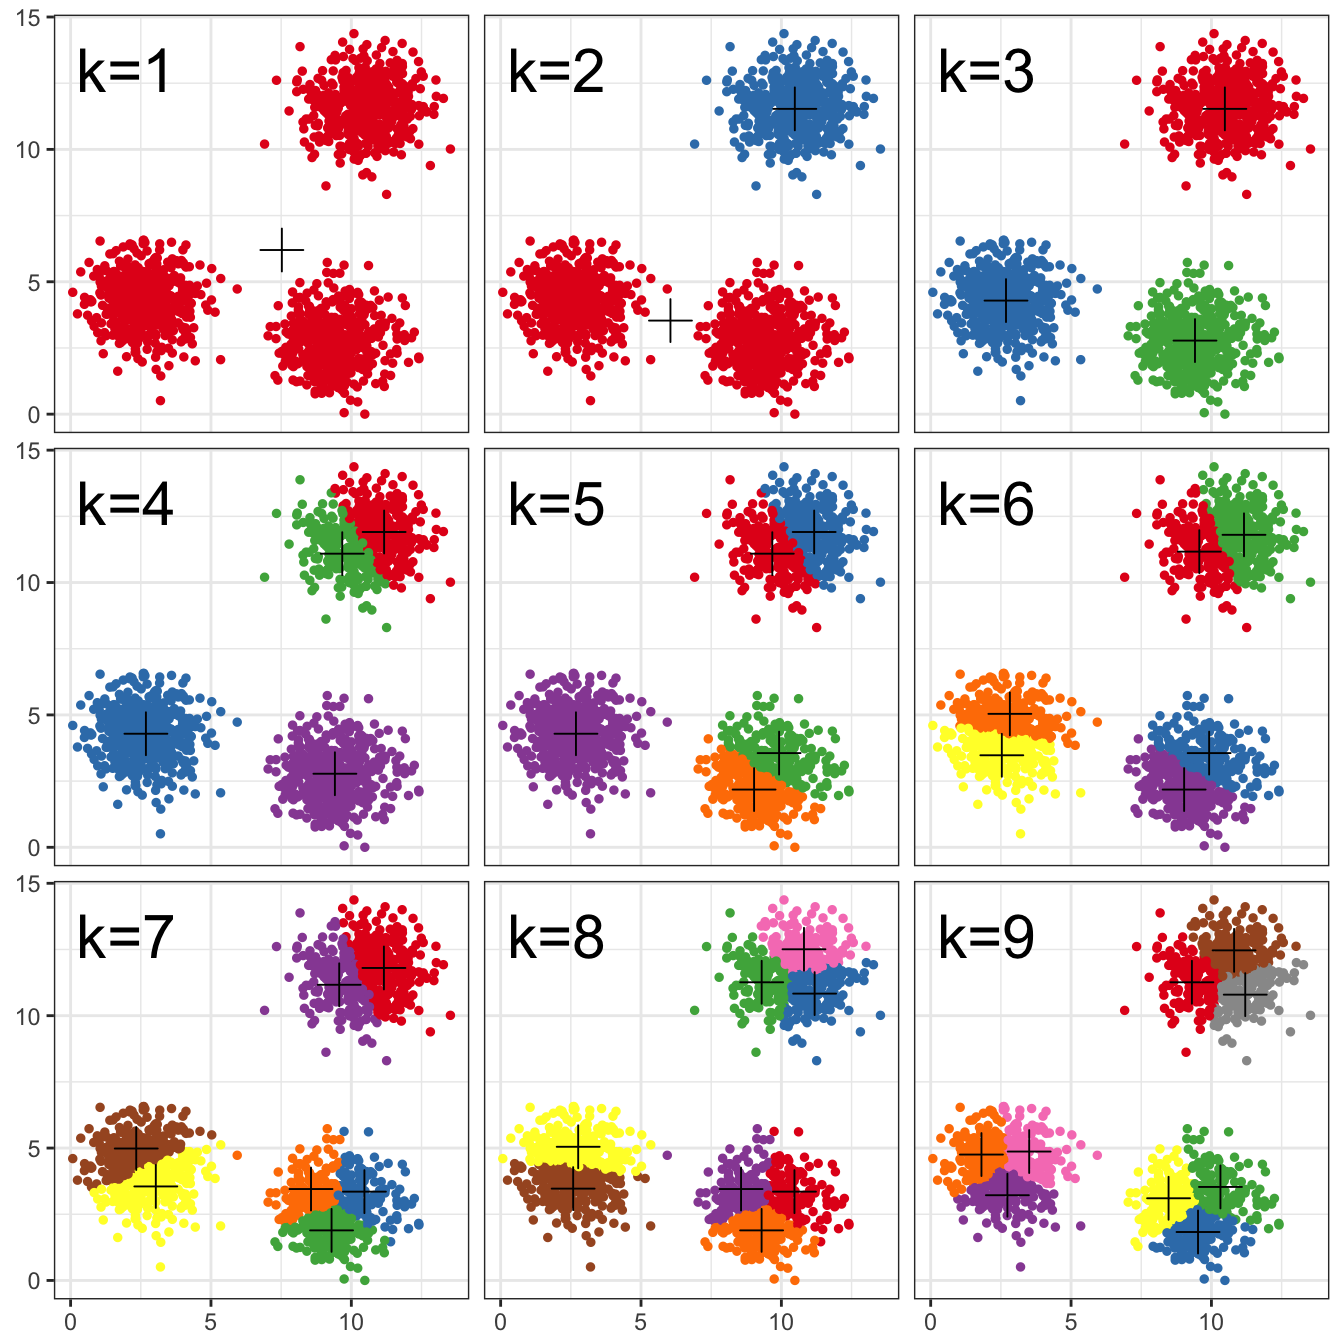
\includegraphics[width=1\linewidth]{09-clustering_files/figure-latex/kmeansRangeK-1} 

}

\caption{K-means clustering of the blobs data set using a range of values of k from 1-9. Cluster centres indicated with a cross.}\label{fig:kmeansRangeK}
\end{figure}

\begin{Shaded}
\begin{Highlighting}[]
\NormalTok{tot_withinss <-}\StringTok{ }\KeywordTok{sapply}\NormalTok{(k, function(i)\{res[[i]]$tot.withinss\})}
\KeywordTok{qplot}\NormalTok{(k, tot_withinss, }\DataTypeTok{geom=}\KeywordTok{c}\NormalTok{(}\StringTok{"point"}\NormalTok{, }\StringTok{"line"}\NormalTok{), }\DataTypeTok{ylab=}\StringTok{"Total within-cluster sum of squares"}\NormalTok{) +}\StringTok{ }\KeywordTok{theme_bw}\NormalTok{()}
\end{Highlighting}
\end{Shaded}

\begin{figure}

{\centering 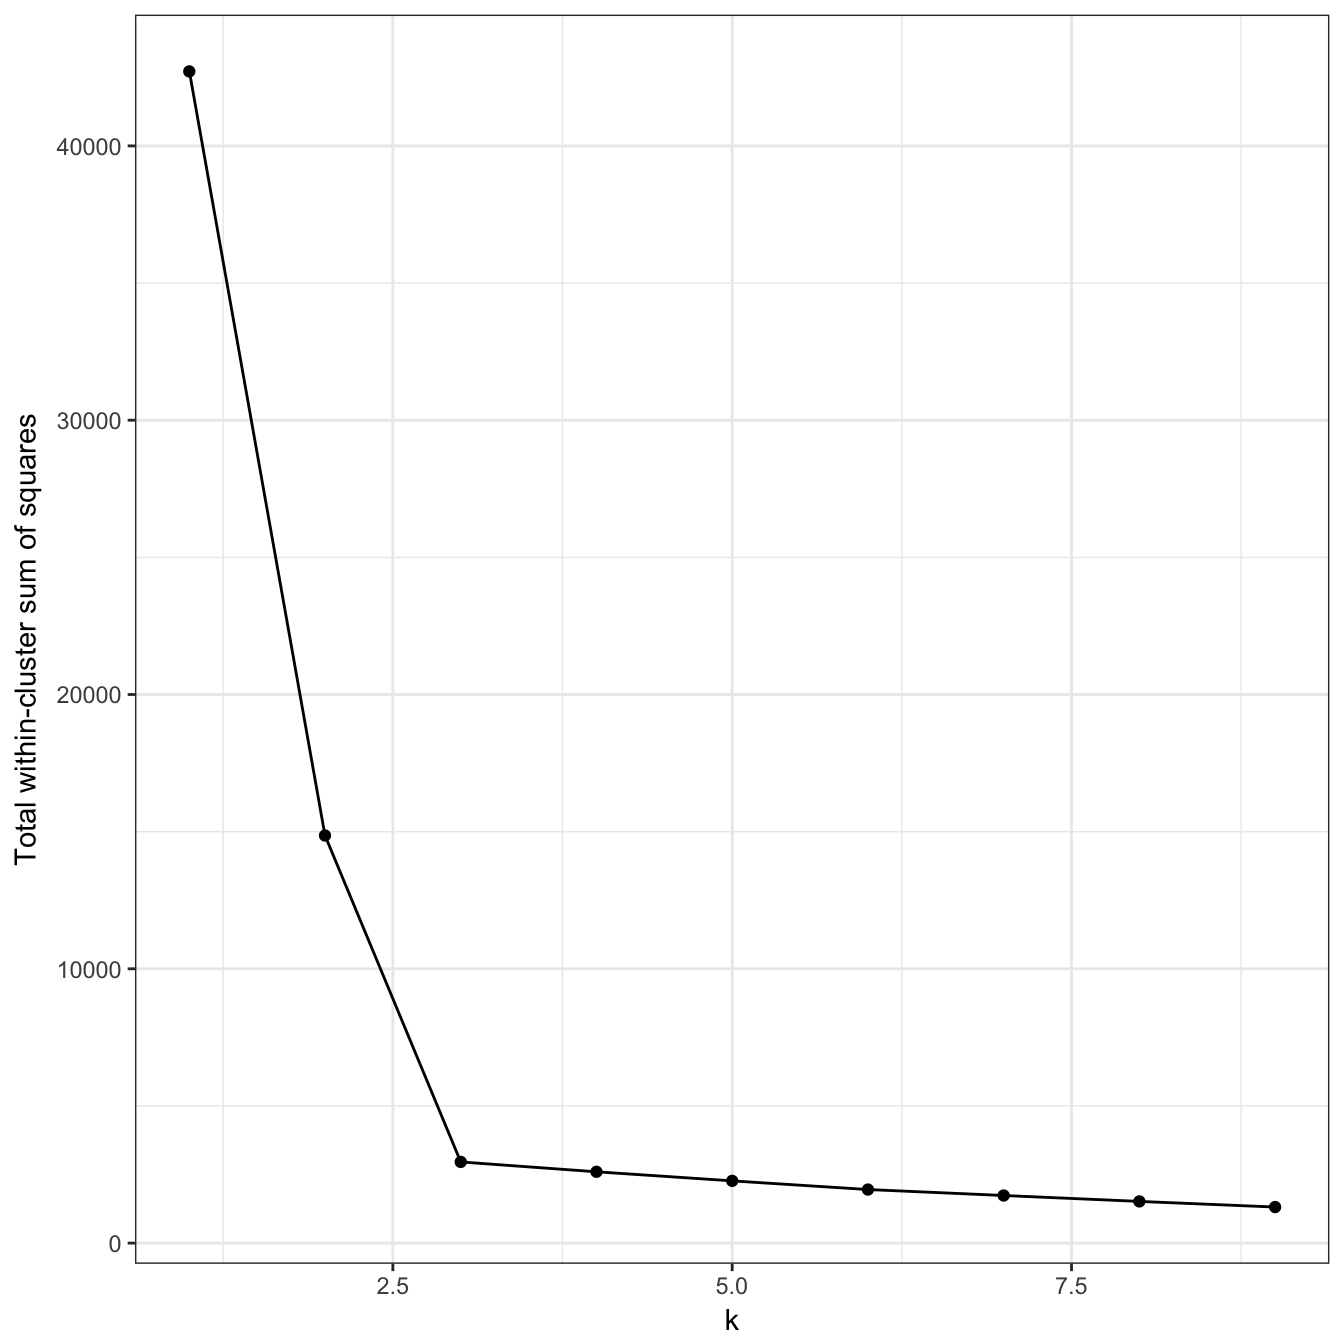
\includegraphics[width=0.5\linewidth]{09-clustering_files/figure-latex/choosingK-1} 

}

\caption{Variance within the clusters. Total within-cluster sum of squares plotted against k.}\label{fig:choosingK}
\end{figure}

\emph{N.B.} we have set \texttt{nstart=50} so that the algorithm is
started 50 times wi

\subsection{DBSCAN}\label{dbscan}

Density-based spatial clustering of applications with noise

\subsubsection{Algorithm}\label{algorithm-1}

Abstract DBSCAN algorithm in pseudocode \citep{Schubert2017}

\begin{verbatim}
1 Compute neighbours of each point and identify core points   // Identify core points
2 Join neighbouring core points into clusters                 // Assign core points
3 foreach non-core point do
      Add to a neighbouring core point if possible            // Assign border points
      Otherwise, add to noise                                 // Assign noise points
\end{verbatim}

\begin{figure}

{\centering 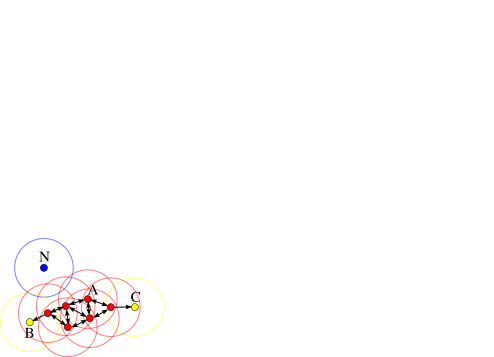
\includegraphics[width=0.75\linewidth]{images/DBSCAN_Illustration} 

}

\caption{Illustration of the DBSCAN algorithm.}\label{fig:dbscanIllustration}
\end{figure}

\subsubsection{Choosing parameters}\label{choosing-parameters}

\subsection{Gene expression}\label{gene-expression}

tissue types?

\section{Summary}\label{summary}

\subsection{Applications}\label{applications}

\subsection{Strengths}\label{strengths}

\subsection{Limitations}\label{limitations}

\section{Exercises}\label{exercises-7}

Exercise solutions: \ref{solutions-clustering}

Solutions to exercises can be found in appendix
\ref{solutions-clustering}.

\appendix


\chapter{Resources}\label{resources}

\section{Python}\label{python}

\href{http://scikit-learn.org}{scikit-learn}

\section{Machine learning data set
repository}\label{machine-learning-data-set-repository}

\href{http://mldata.org/}{mldata.org}

This repository manages the following types of objects:

\begin{itemize}
\tightlist
\item
  Data Sets - Raw data as a collection of similarily structured objects.
\item
  Material and Methods - Descriptions of the computational pipeline.
\item
  Learning Tasks - Learning tasks defined on raw data.
\item
  Challenges - Collections of tasks which have a particular theme.
\end{itemize}

\chapter{Solutions ch.~3 - Linear models and matrix
algebra}\label{solutions-linear-models}

Solutions to exercises of chapter \ref{linear-models}.

\section{Exercise 1}\label{exercise-1}

\section{Exercise 2}\label{exercise-2}

\chapter{Solutions ch.~4 - Linear and non-linear logistic
regression}\label{solutions-logistic-regression}

Solutions to exercises of chapter \ref{logistic-regression}.

\section{Exercise 1}\label{exercise-1-1}

\section{Exercise 2}\label{exercise-2-1}

\chapter{Solutions ch.~5 - Nearest
neighbours}\label{solutions-nearest-neighbours}

Solutions to exercises of chapter \ref{nearest-neighbours}.

\section{Exercise 1}\label{exercise-1-2}

\section{Exercise 2}\label{exercise-2-2}

\chapter{Solutions ch.~6 - Decision trees and random
forests}\label{solutions-decision-trees}

Solutions to exercises of chapter \ref{decision-trees}.

\section{Exercise 1}\label{exercise-1-3}

\section{Exercise 2}\label{exercise-2-3}

\chapter{Solutions ch.~7 - Support vector machines}\label{solutions-svm}

Solutions to exercises of chapter \ref{svm}.

\section{Exercise 1}\label{exercise-1-4}

\section{Exercise 2}\label{exercise-2-4}

\chapter{Solutions ch.~8 - Artificial neural
networks}\label{solutions-ann}

Solutions to exercises of chapter \ref{ann}.

\section{Exercise 1}\label{exercise-1-5}

\section{Exercise 2}\label{exercise-2-5}

\chapter{Solutions ch.~9 - Dimensionality
reduction}\label{solutions-dimensionality-reduction}

Solutions to exercises of chapter \ref{dimensionality-reduction}.

\section{Exercise 1}\label{exercise-1-6}

\section{Exercise 2}\label{exercise-2-6}

\chapter{Solutions ch.~10 - Clustering}\label{solutions-clustering}

Solutions to exercises of chapter \ref{clustering}.

\section{Exercise 1}\label{exercise-1-7}

\section{Exercise 2}\label{exercise-2-7}

\bibliography{packages.bib,book.bib}


\end{document}
